\documentclass[14pt]{extarticle}

\usepackage[utf8]{inputenc}
\usepackage[T2A,T1]{fontenc}
\usepackage[russian]{babel}
\usepackage[a4paper,lmargin=3cm,rmargin=2cm,tmargin=2cm,bmargin=2cm]{geometry}
\usepackage[ddmmyyyy]{datetime}
\usepackage{indentfirst}
\usepackage{hyperref}
\usepackage{graphicx}
\graphicspath{{./images/}}

\usepackage{minted}

\usepackage{titlesec}
\titleformat{\section}{\normalfont\bfseries\centering}{\thesection}{1em}{}
\titleformat{\subsection}{\normalfont\bfseries}{\thesubsection}{1em}{}
\usepackage{setspace}
\singlespacing
%\onehalfspacing
%\doublespacing
\setlength{\parindent}{1.25cm}
\let\oldsection\section
\renewcommand\section{\clearpage\oldsection}

\usepackage[backend=biber]{biblatex}
\addbibresource{~/texdoc/bibl.bib}
\input{~/texdoc/unibind.tex}
\usepackage{multirow}

\usepackage{pgf}
\usepackage{tikz}
\usetikzlibrary{arrows,automata}
\usetikzlibrary{positioning}

\tikzset{
	state/.style={
		rectangle,
		draw=black, very thick,
		anchor=west, align=left,
		text width=6cm,
	},
}
\usepackage{csquotes}
\usepackage{mathtools}

\begin{document}
\unititle
{\klgtu}
{\fapu}
{\suvt}
{Лабораторная работа №1 \par Структурный и функциональный анализ систем}
{По дисциплине: «Надежность и качество АСОИУ»}
{Доцент}
{Розен Н.Б.}
{ст. гр. 18-ВТ}
{Поляков Л.Д.}

\tableofcontents

\section{Задание}

Для объекта: Автоматизированная система – Учета товаров на складе выполнить следующие работы:
\begin{enumerate}
	\item Построение иерархии системы;
	\item Описание сущностных свойств системы;
	\item Описание функционирования системы в пространстве состояний
	\item Описание управления системой.
	\item Выполнение необходимых графических работ, заполнение необходимых таблицы, подготовка и представление отчета о проделанной работе.
\end{enumerate}

\section{Ход работы}

\subsection{Построение иерархии системы}

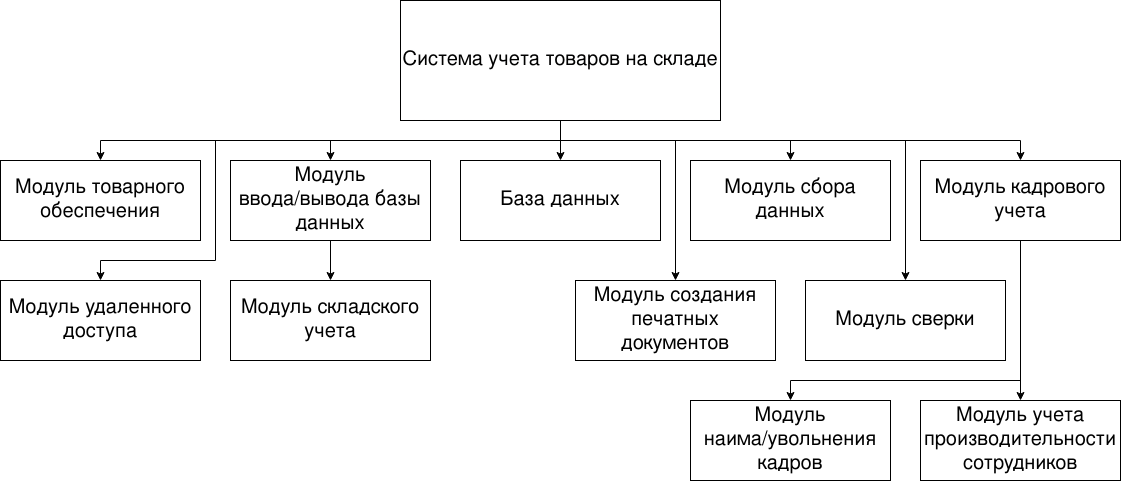
\includegraphics[width=\textwidth]{MonitorF.drawio}

\subsection{Описание сущностных свойств системы}

Система имеет свойство автоматизированного управления складом с возможностью удаленного просмотра базы данных.

\subsection{Описание функционирования системы в пространстве состояний}

% Исправное, работоспособное и рабочее состояние, 

Состояние каждого элемента в одной определенной ситуации

\begin{tabular}{|p{0.15\textwidth}|p{0.18\textwidth}|p{0.24\textwidth}|p{0.18\textwidth}|}
	\hline
Состояние сетевого подключения & Исправное & Работоспособное & Рабочее \\ \hline
Состояние электричества & Исправное & Работоспособное & Рабочее \\ \hline
Состояние сотрудников & Исправное & Работоспособное & Рабочее \\ \hline
Состояние базы данных  & Исправное & Работоспособное & Рабочее \\ \hline
\end{tabular}

\subsection{Описание управления системой}

% Управление и взаимодействие с внешней средой

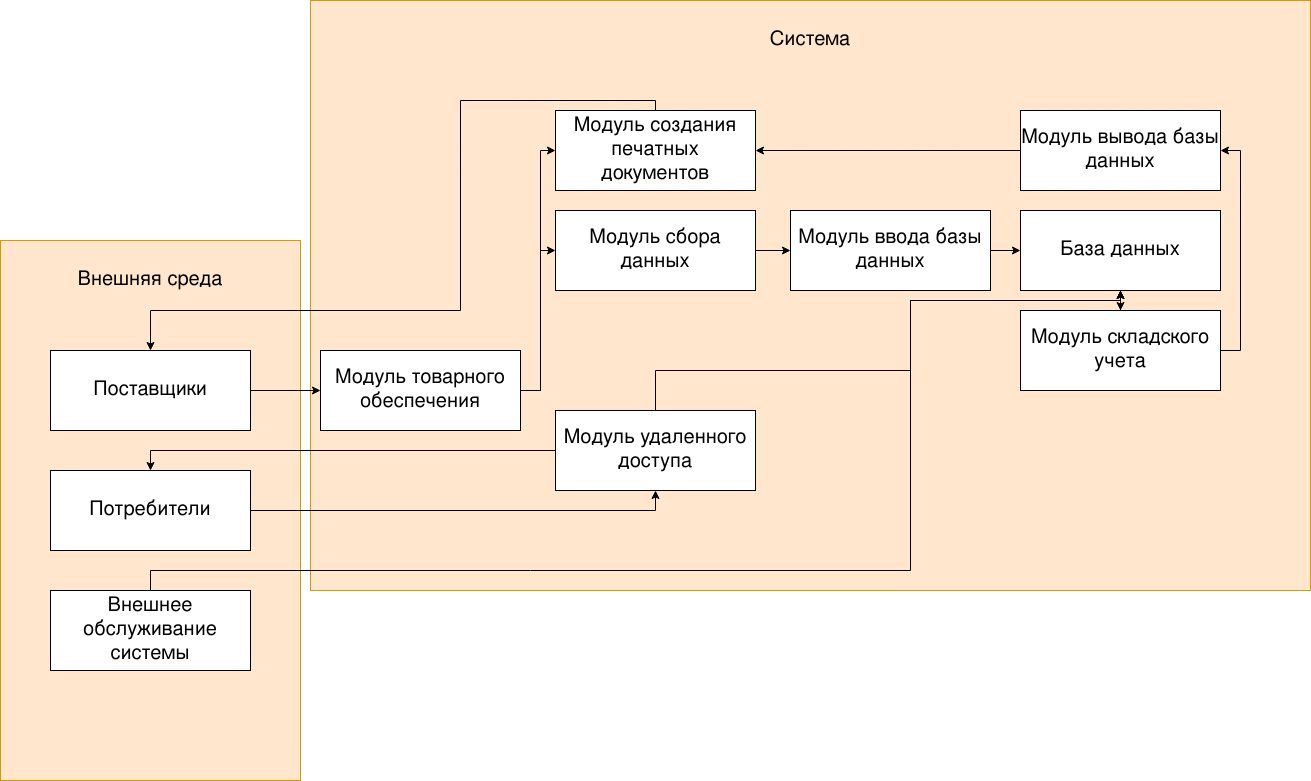
\includegraphics[width=\textwidth]{External.drawio}




\end{document}
